\pdfminorversion=4
\documentclass[presentation, aspectratio=54]{beamer}
\usepackage[utf8]{inputenc}
\usepackage[T1]{fontenc}
\usepackage{graphicx}
\usepackage{float}
\usepackage{wrapfig}
\usepackage[normalem]{ulem}
\usepackage{amsmath}
\usepackage{bm}
\usepackage{textcomp}
\usepackage{amssymb}
\usepackage{hyperref}
\usepackage{textgreek}
\usepackage[backend=biber,style=numeric-comp,sorting=none]{biblatex}
\addbibresource{ref.bib}
\tolerance=1000
% Include this file for light background SUTD style
% Version 1: Nils Ole Tippenhauer, SUTD, 2014
% Version 2: Sibo Song, SUTD, 2016
\mode<presentation>

\usecolortheme{rose}
\useinnertheme{rounded}
\usecolortheme{dolphin}
\useoutertheme{infolines}

% more stuff from Boadilla sty
\setbeamersize{text margin left=1.5em,text margin right=1.5em}
% disables headline
\setbeamertemplate{headline}[default]
\mode<all>

% resize footnote font size
\setbeamerfont{footnote}{size=\tiny}

% disable tool bar
\beamertemplatenavigationsymbolsempty

% logo. If your logo has different dimension, this might need tweaking
\usepackage{pgf}  
\logo{\pgfputat{\pgfxy(-1,8)}{\pgfbox[center,base]{
\includegraphics[height=1.2cm]{figure/SUTDMainLogo.png}}}}

% fonts
\usepackage{helvet}
\usepackage{times}
\usefonttheme{serif}

% title page, simple version
\setbeamertemplate{title page}{
{\usebeamerfont{title}\LARGE\bf\inserttitle\vspace{0.1cm}\hrule}
\vspace{0.2cm}\usebeamerfont{author}\hfill\insertauthor
}

% color
\definecolor{SUTDred}{RGB}{153,0,51}
\definecolor{white}{RGB}{255,255,255}
\definecolor{lgrey}{RGB}{204,204,204}
\definecolor{mgrey}{RGB}{102,102,102}
\definecolor{dgrey}{RGB}{51,51,51}

% hline for the titles
\setbeamertemplate{frametitle}{
\vspace{0.2cm}
{\usebeamerfont{title}\bf\insertframetitle\par\vskip-6pt\line(1,0){275}}}

% set text color 
\setbeamercolor{normal text}{fg=black,bg=white}
\setbeamercolor{section number projected}{fg=black}
\setbeamercolor{section in toc}{fg=black}
\setbeamercolor{title}{fg=black}
\setbeamercolor{frametitle}{fg=black}
\setbeamercolor{framesubtitle}{fg=black}
\setbeamercolor{caption}{fg=black}

% highlight color using \alert{} command
\setbeamercolor{alerted text}{fg=SUTDred}

% set items styles to be default
% \setbeamertemplate{itemize items}[default]
% \setbeamertemplate{enumerate items}[default]

% item color setting
\setbeamercolor{item}{fg=black,bg=lgrey}
\setbeamercolor{item projected}{use=item,fg=black,bg=item.fg!35}
\setbeamercolor{subitem}{fg=black,bg=mgrey}
\setbeamercolor{subitem projected}{use=item,fg=black,bg=item.fg!35}

% itemize item style setting
\useitemizeitemtemplate{\Large\hbox{\textbullet}}
\usesubitemizeitemtemplate{\tiny\hbox{$\blacktriangleright$}}
\usesubsubitemizeitemtemplate{\tiny\hbox{$\star$}}

% enumerate item style setting
\setbeamertemplate{enumerate item}{\insertenumlabel.}
\setbeamertemplate{enumerate subitem}{\alph{enumii}.}
\setbeamertemplate{enumerate subsubitem}{(\alph{enumiii}).}
\setbeamertemplate{enumerate mini template}{\insertenumlabel}

% palette color setting
\setbeamercolor{palette primary}{fg=white,bg=SUTDred}
\setbeamercolor{palette secondary}{fg=white,bg=mgrey}
\setbeamercolor{palette tertiary}{fg=black,bg=lgrey}
\setbeamercolor{palette quaternary}{fg=white,bg=lgrey} 

% block color setting
\setbeamercolor{block title}{fg=black,bg=black!15}
\setbeamercolor{block body}{fg=black,bg=black!5}
\setbeamercolor{block title alerted}{parent=alerted text,bg=black!15}
\setbeamercolor{block title example}{parent=example text,bg=black!15}


\usetheme{default}
\author{Author name}
\date{April 29, 2016}
\title[short title]{Slides template \LaTeX - SUTD theme}
\begin{document}

\maketitle
%-----------------------------------------------------

\begin{frame}{List}

\begin{columns}
\begin{column}{0.5\textwidth}
\begin{enumerate}
\item \alert{enumerate}
  \begin{enumerate}
  \item sub item a
    \begin{enumerate}
    \item sub sub item alpha
    \item sub sub item beta
    \item sub sub item gamma
    \end{enumerate}
  \item sub item b
  \item sub item c
  \end{enumerate}
\end{enumerate}
\end{column}

\begin{column}{0.5\textwidth}
\begin{itemize}
\item \alert{itemize}
  \begin{itemize}
  \item sub item
    \begin{itemize}
    \item sub sub item
    \item sub sub item
    \item sub sub item
    \end{itemize}
  \item sub item
  \item sub item
  \end{itemize}
\end{itemize}

\end{column}
\end{columns}

\end{frame}
%-----------------------------------------------------

\begin{frame}{Blocks}
\begin{block}{Block 1}
This is a normal block.
\end{block}
\begin{exampleblock}{Block 2}
This is an example block.
\end{exampleblock}
\begin{alertblock}{Block 3}
This is an alert block.
\end{alertblock}
\end{frame}
%-----------------------------------------------------

\begin{frame}{Figure and Reference}

\begin{center}
\begin{figure}
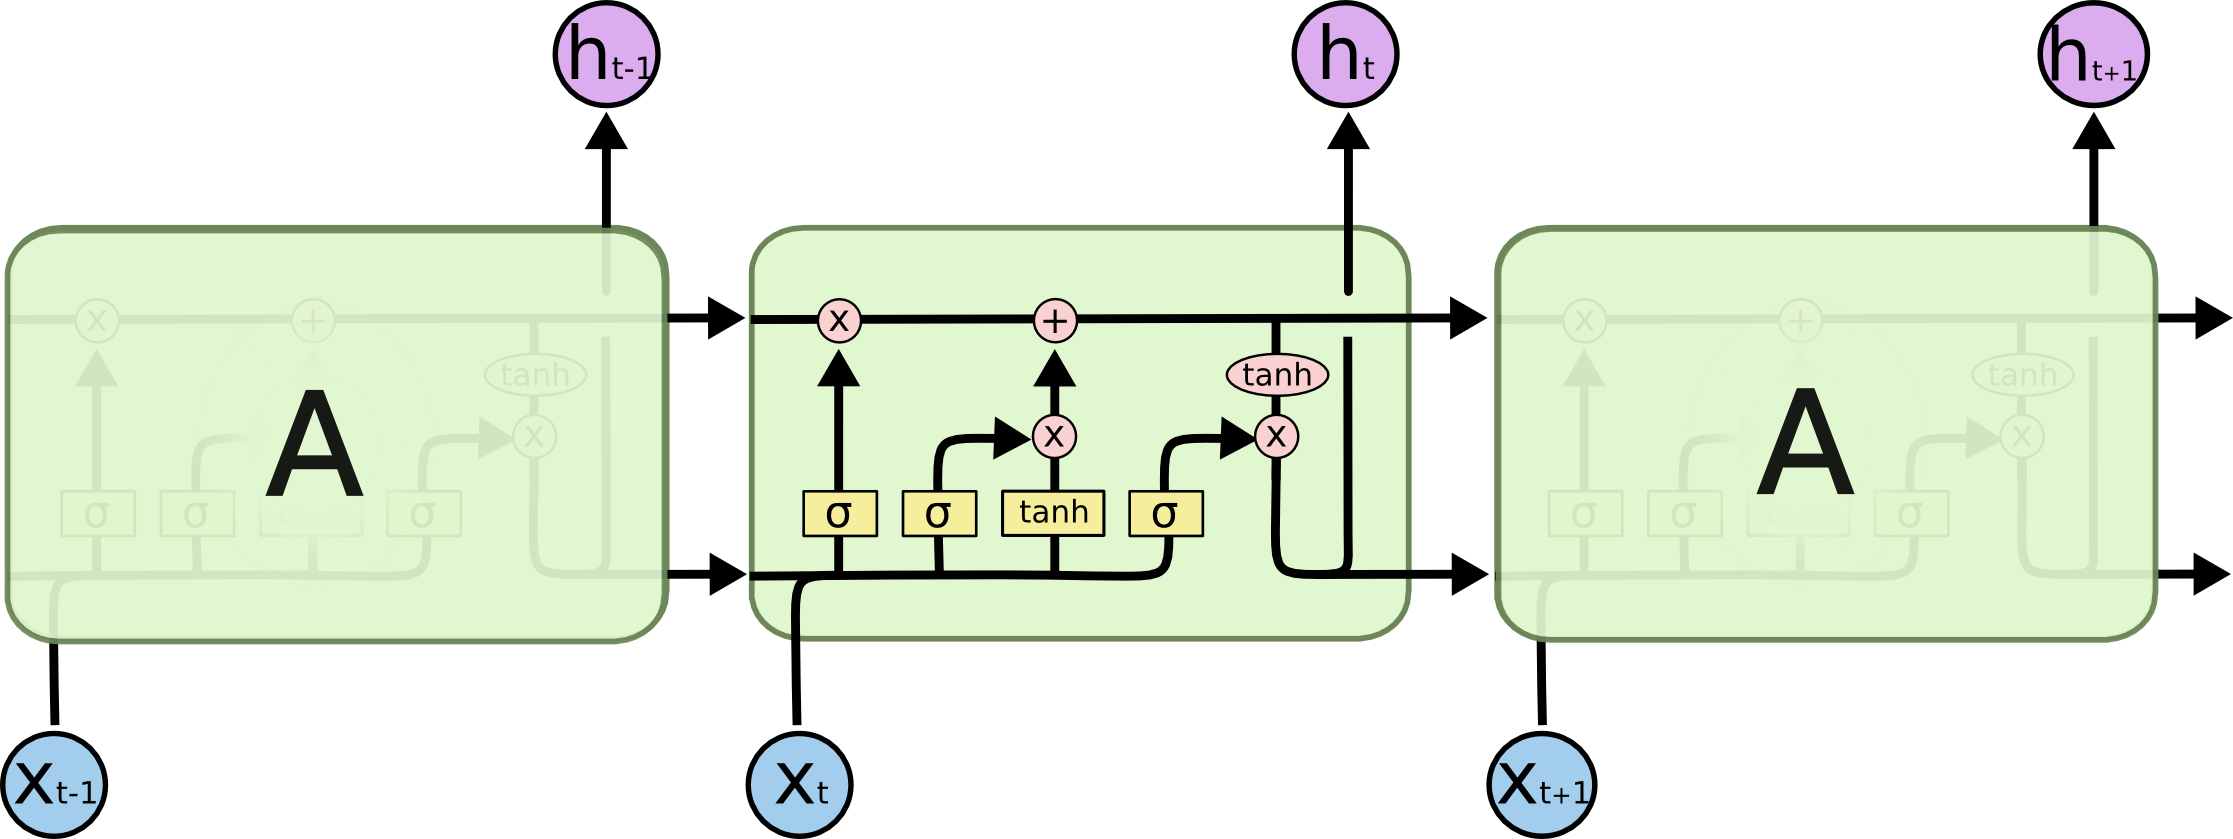
\includegraphics[width=0.9\linewidth]{figure/LSTM3-chain.png}
\caption{LSTM Diagram \footfullcite{understandLSTM}}
\label{fig:campus}
\end{figure}
\end{center}

\end{frame}
%-----------------------------------------------------

\begin{frame}{Equation and Table}

\begin{columns}
\begin{column}{0.5\textwidth}
\begin{align*}
i &=\sigma(x_tU^i + h_{t-1} W^i) \\
f &=\sigma(x_t U^f +h_{t-1} W^f) \\  
o &=\sigma(x_t U^o + h_{t-1} W^o) \\  
g &=\tanh(x_t U^g + h_{t-1}W^g) \\  
c_t &= c_{t-1} \circ f + g \circ i \\  
h_t &=\tanh(c_t) \circ o  
\end{align*}  
\end{column}

\begin{column}{0.5\textwidth}
% Table
\begin{table}[]
\centering
\caption{Sample Table}
\label{tab:sample}
\scalebox{0.8}{
\begin{tabular}{c|c|c}
Year         & stats 1      & stats 2      \\ \hline \hline
2013         & 41.5\%       & 46.0\%       \\ \hline
2014         & 38.0\%       & 48.0\%       \\ \hline
2015         & 40.0\%       & 53.5\%       \\  
\end{tabular}}
\end{table}
\end{column}
\end{columns}

\end{frame}
%-----------------------------------------------------

\begin{frame}
\begin{center}
\Huge Thank You!
\end{center}
\end{frame}
%-----------------------------------------------------

\end{document}